Concurrent Red-Black tree is used in crucial places inside operating system kernels like Virtual Memory(VM) region trees where they have great impact on scalability of multithreaded VM-intensive applications.  We analyse this important data
structure under RCU semantics and we try to explore free linearisability properties when we apply our type system. 

\textsf{\textbf{Readers}}. With RCU technique developing a reader is almost as easy as developing a non-concurrent reader.  The only restrictions placed on readers are that they do not hold any references to the data structure outside critical section.


\textsf{\textbf{Mutators}}. Lock-free proceeding of \textsf{Readers} can be provided with keeping Red-Black tree consistent by \textsf{Mutators}. 
\begin{itemize}
\item Mutator must not allow a reader to see partial changes to a node. Mutator use copy-on-update to make all changes to a private copy of the node, then atomically switch the new node with the old one.
\item Readers must not get lost when the structure of the tree is changed. In the Zig restructure below, if a reader is at node \textsf{A} looking for node \textsf{B} at the same time the restructure happens, the reader will never find \textsf{B}. The reason is after restructure
	we have \textsf{B} is above \textsf{A} instead of below it. 
\item Discuss with Matt: Temporarily having the same item in the tree multiple times won't affect the lookups. A unique value is returned if first copy encountered and another unique value can be returned if second copy is encountered.
\end{itemize}

% Restructure operations to rebalance a red black tree. There are left and right versions of these, but they are symmetric so only the left version is shown here.
\begin{figure}
\centering
\[
\begin{array}{r@{\;\;\Longrightarrow_{transform}\;\;}ll}

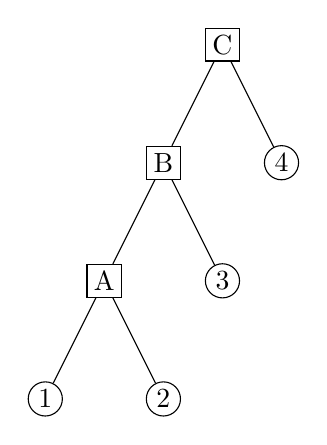
\begin{tikzpicture}
\tikzstyle{hollow node}=[circle,draw,inner sep=1.5]
\tikzstyle{solid node}=[rectangle,draw,inner sep=2.5]
\tikzset{
	red node/.style={circle,draw=red,fill=red,inner sep=2.2},
	blue node/.style={rectangle,draw=blue,inner sep=2.5}
}
\node[solid node]{C}
	child{
		node[solid node]{B}			
			child{node[solid node]{A}
					child{node[hollow node]{1}}
					child{node[hollow node]{2}}					
			}
			child{node[hollow node]{3}}
	}
	child{node[hollow node]{4}}
	
;
\end{tikzpicture}
&
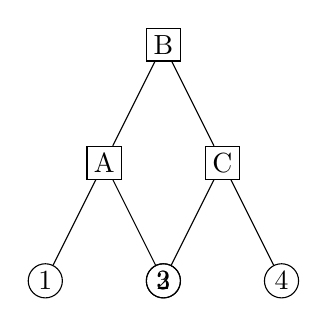
\begin{tikzpicture}
\tikzstyle{hollow node}=[circle,draw,inner sep=1.5]
\tikzstyle{solid node}=[rectangle,draw,inner sep=2.5]
\tikzset{
	red node/.style={circle,draw=red,fill=red,inner sep=2.2},
	blue node/.style={rectangle,draw=blue,inner sep=2.5}
}
\node[solid node]{B}
			child{node[solid node]{A}
					child{node[hollow node]{1}}
					child{node[hollow node]{2}}					
			}
			child{node[solid node]{C}
					 child{node[hollow node]{3}} 
					 child{node[hollow node]{4}}
			}		
			
;
\end{tikzpicture}
&
 \textrm{Diag Structure}
\\
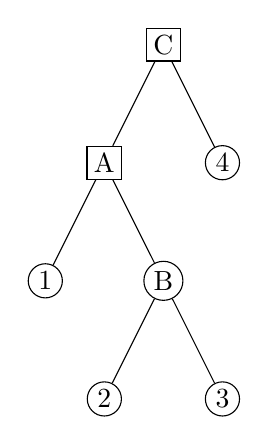
\begin{tikzpicture}
\tikzstyle{hollow node}=[circle,draw,inner sep=1.5]
\tikzstyle{solid node}=[rectangle,draw,inner sep=2.5]
\tikzset{
	red node/.style={circle,draw=red,fill=red,inner sep=2.2},
	blue node/.style={rectangle,draw=blue,inner sep=2.5}
}
\node[solid node]{C}							
			child{node[solid node]{A}
					child{node[hollow node]{1}}
					child{node[hollow node]{B}
								child{node[hollow node]{2}}
								child{node[hollow node]{3}}
					}							
			}					
			child{node[hollow node]{4}}	
	
	
;
\end{tikzpicture}
&
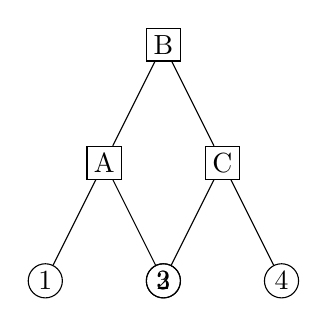
\begin{tikzpicture}
\tikzstyle{hollow node}=[circle,draw,inner sep=1.5]
\tikzstyle{solid node}=[rectangle,draw,inner sep=2.5]
\tikzset{
	red node/.style={circle,draw=red,fill=red,inner sep=2.2},
	blue node/.style={rectangle,draw=blue,inner sep=2.5}
}
\node[solid node]{B}
			child{node[solid node]{A}
					child{node[hollow node]{1}}
					child{node[hollow node]{2}}					
			}
			child{node[solid node]{C}
					 child{node[hollow node]{3}} 
					 child{node[hollow node]{4}}
			}		
			
;
\end{tikzpicture}
&
 \textrm{Zig Structure}
\\

\end{array}
\]
\caption{Restructure operations used to rebalance a red black tree. There are left and right versions of these, but they are symmetric so only the left version is shown here.}
\end{figure}

\subsubsection{Swap}
Consider the delete of node \textsf{B} shown in  below. Since \textsf{B} is an internal, \textsf{B} will be swapped with \textsf{C} $(= next ($ \textsf{B} )$)$ prior to deletion.
\newpage

\begin{figure}
\centering
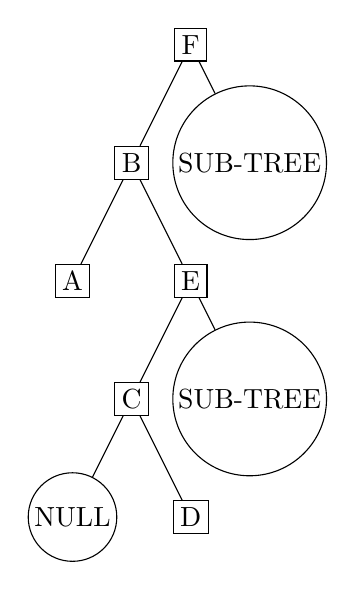
\begin{tikzpicture}
\tikzstyle{hollow node}=[circle,draw,inner sep=1.5]
\tikzstyle{solid node}=[rectangle,draw,inner sep=2.5]
\tikzset{
	red node/.style={circle,draw=red,fill=red,inner sep=2.2},
	blue node/.style={rectangle,draw=blue,inner sep=2.5}
}
\node[solid node]{F}
			child{node[solid node]{B}
					child{node[solid node]{A}}
					child{node[solid node]{E}
							child{node[solid node]{C}
								child{node[hollow node]{NULL}}
								child{node[solid node]{D}}
							}
							child{node[hollow node]{SUB-TREE}}	
					}					
			}
			child{node[hollow node]{SUB-TREE}}						
;
\end{tikzpicture}
\caption{Tree Before Deletion of node B}
\end{figure}



\textsf{C'} is allocated with color and children of B, but with key and data  values of C.  The \textsf{C'} is linked into tree as in place of \textsf{B}. The value of \textsf{C} can be  observed twice in tree. In this setting, readers who are below \textsf{B} and above \textsf{C'} can read the value of \textsf{C} safely.
This is because \textsf{C} is kept until all readers below \textsf{B} looking for value of \textsf{C} is are done. In other words, garbage collector thread waits for a grace period before removing \textsf{C} from the tree. This preserves that readers below \textsf{B} will complete their read prior to \textsf{C} being removed.

\begin{figure}
\centering
\begin{tikzpicture}[>=stealth',node distance=2.5cm,semithick,auto]
\tikzstyle{hollow node}=[circle,draw,inner sep=1.5]
\tikzstyle{sub node}=[triangle,draw,inner sep=1.5]
\tikzstyle{solid node}=[rectangle,draw,inner sep=2.5]

\tikzset{
	red node/.style={rectangle,draw=red,fill=red,inner sep=2.2},
	blue node/.style={rectangle,draw=blue,inner sep=2.5}
}
    \node[solid node]                  (F)                             {$F$};
    \node[solid node]            (Cp)    [below left of=F]            {$C'$};
    \node[red node]            (B)    [right of=Cp]           {$B$};
   \node[solid node]            (A)    [below left of=Cp]     {$A$};
    \node[solid node]            (E)    [below right of=B]           {$E$};
    \node[red node]            (C)    [below left of=E]     {$C$};
    \node[solid node]            (D)    [below right of=C]           {$D$};
    \node[hollow node]            (N)    [below left of=C]     {$NULL$};
    \node[hollow node]            (STF)  [right of= F] {$SUB-TREE$};
   \node[hollow node]            (STE)  [ right of= E] {$SUB-TREE$};

    \path[-]   (F)     edge                        node        {}              (Cp)
                (Cp)    edge                        node        {}    (A)
                (Cp)    edge                        node        {}    (E)
                (B)    edge                        node        {}    (A)
                (B)    edge                        node        {}    (E)
                (E)    edge                        node        {}    (D)
                (C)    edge                        node        {}    (D)
                (C)    edge                        node        {}    (N)
		(E)	edge				node		{}	(STE)
		(F)	edge				node 	{}	(STF)
;
\end{tikzpicture}
\caption{Tree after deletion of node B. The red nodes are scheduled for reclamation.}
\end{figure}
[TODO: Informal Reasonings on Rotations, Evaluation Order]
